%%%% PROCESAR con PdfLaTeX !!!!!


\documentclass[12pt]{book}
\usepackage{geometry}\geometry{top=2cm,bottom=2cm,left=3cm,right=3cm}
\usepackage{amssymb}
\usepackage{amsmath}
\usepackage{graphicx}
\usepackage{txfonts}




\begin{document}
\thispagestyle{empty}

\begin {center}

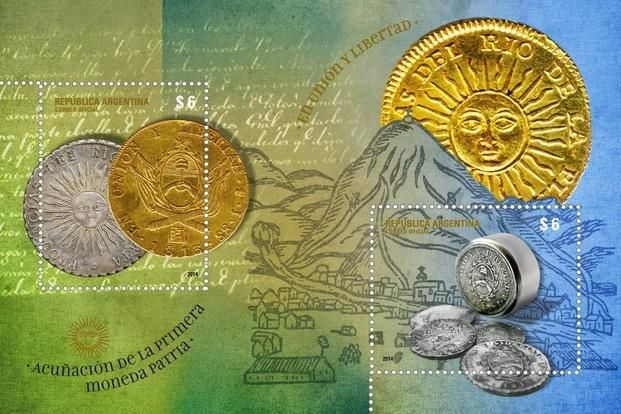
\includegraphics[scale=.4]{1484058646033.jpg}

\medskip
UNIVERSIDAD DE BUENOS AIRES

Facultad de Econom\'ia


\vspace{3cm}


\textbf{\large HISTORIA ECONOMICA SOCIAL GENERAL}

\vspace{2cm}


Este es un compendio de apuntes de clase, resumenes de la bibliograf\'ia obligatoria y es un aporte para los alumnos y los interesados en general.
De ninguna man\'era pretende ser una gu\'ia de estudio, ni remplaza las clases presenciales, el material oficial de la catedra esta disponible en el web site de la m\'ateria.
\\

\end {center}


\vspace{2.5cm}

\noindent Autor:\,	Isaac Edgar Camacho Ocampo
 
\noindent Carrera:\,	Licenciado en Econom\'ia

\vspace{1cm}

\vspace{1cm}

\noindent Buenos Aires, 2019

\newpage


\tableofcontents

\tableofcontents
\chapter{Revoluci\'on industrial}
\section{¿En que consistio la revolucion industrial?}
Capitulo 3,5 del libro de Barbero
 Comenzaremos con la siguiente interrogante ¿cual es el significado que los historiadores le atribuyen hoy al termino RI? Como vimos anteriormente no existe un consenzo entre los diferentes autores.
 \\
\\
\textbf{David landes propone 3 definiciones}
\begin{itemize}
 \item \textbf{revolucion industrial} en minuscula, se refiere al complejo de innovaciones tecnol\'ogicas que al sustituir la habilidad humana por maquinaria y la fuerza humana y animal por energ\'ia mec\'anica, provoca el paso desde un tipo de producci\'on artesanal a un tipo de producci\'on fabril naciendo as\'i la econom\'ia moderna.
 \item Otro significado que suele atribuirse al t\'ermino \textbf{Revoluci\'on Industrial}  es para referirse a cualquier proceso de cambio tecnol\'ogico r\'apido e importante.	En este sentido se habla tambien de una segunda y tercera revoluci\'on entendidas como una secuancia de innovaci\'on industrial historicamanete determinadas.
 \item \textbf{REVOLUCI\'ON INDUSTRIAL} con may\'uscula se refiere a la primera circunstancia hist\'orica de cambio desde una econom\'ia de base agraria y artesanal a otra dominada por la industria y la manufactura mecanizada, en este sentido la RI se inici\'o en inglaterra en el siglo XVIII y se expandio desde all\'i a los paises de la europa continental adem\'as de otras areas y transformo en menos de dos generaciones la vida del hombre occidental la naturaleza de su sociedad y sus relaciones con los demas pueblos.
 \end{itemize} 
\textbf{Por otro lado en historiador ingl\'es Peter Mathias} define la RI como (las fases iniciales del proceso de industrializaci\'on en el largo plazo), y señala dos criterios esenciales para definirla.
\begin{enumerate}
\item La aceleraci\'on del crecimiento de la econom\'ia en su conjunto.
\item Cambios estructurales.
\end{enumerate}

\section{Estado del arte}
\chapter{Fundamentos teóricos}
\section{Teoría clásica}
\subsection{Definición de variables}
\subsection{Pruebas y refutaciones}
\section{Hipótesis}
\chapter{Resultados}
\section{Simulación de resultados}
\subsection{Suposiciones}
\subsection{Modelos}
\section{Resultados preliminares}
\section{Resultados postprocesados}
\subsection{Valores atípicos}
\subsection{Correlaciones}
\chapter{Conclusiones}
\end{document}
